\documentclass[10pt,lettersize,journal]{IEEEtran}
\usepackage{fontspec}
\IfFontExistsTF{Times New Roman}{\setmainfont{Times New Roman}}{\setmainfont[BoldFont=texgyretermes-bold.otf,ItalicFont=texgyretermes-italic.otf,BoldItalicFont=texgyretermes-bolditalic.otf]{texgyretermes-regular.otf}}
\usepackage{amsmath,amssymb,graphicx,booktabs,url}
\usepackage[hidelinks]{hyperref}
\newsavebox{\uploadedtablebox}
\renewcommand{\thetable}{S\arabic{table}}
\title{Supplemental Material: Regional Complementarity and Learned Weighting for Occluded Face Verification}
\author{Sangiya Pararajasingham}
\renewcommand{\thefigure}{S\arabic{figure}}
\begin{document}
\maketitle
\noindent\textit{References: main-paper numbering.}\par

\section{Parameter efficiency}

M0 has 590,592 trainable parameters. M2 contains an unused full face branch. Its active periocular branch has 1,032,960 trainable parameters. 2,065,920 is the nominal trainable parameter count of the instantiated model. The 128-class training-only head has 98,432 parameters and is not included in this table. Across all adapted models, the maximum number of trainable parameters is 2.26M (1.29\%), within a double encoder model (175M). Hardware details, available runtimes, software versions, and checkpoint hashes are recorded in the artifact. Peak memory consumption was not measured.\par

\begin{table}[t]\centering
\caption{Total model parameters and the proportion trainable. The training-only classifier head is not included.}
\label{tab:checked2}
\footnotesize\setlength{\tabcolsep}{2pt}
\sbox{\uploadedtablebox}{\begin{tabular}{llll}\toprule
ID & Total Parameters & Trainable Parameters & (\%) Trainable\\\midrule
M0 & 87171072 & 590592 & 0.68\\
M1 & 87613440 & 1032960 & 1.18\\
M2 & 175226880 & 2065920 & 1.18\\
M3 & 175226880 & 2065920 & 1.18\\
M4 & 175424257 & 2263297 & 1.29\\
\bottomrule\end{tabular}}
\ifdim\wd\uploadedtablebox>\columnwidth\resizebox{\columnwidth}{!}{\usebox{\uploadedtablebox}}\else\usebox{\uploadedtablebox}\fi
\end{table}

\section{Execution and recovery records}

Execution environment: PyTorch (version 2.14.0+cpu), deterministic. DINOv2 was cached. Checkpoints are saved atomically and contain optimiser state, ordered data samples, next batch index, loss in current epoch, and random number generator states in Python, NumPy and PyTorch. Incompatible checkpoints cannot be resumed because manifest and source signatures are checked. Before the serial co-ordinator retains a run as complete, all recorded hash checks must pass. Periocular only training means that full face encoder was not used in forward passes. This means that random numbers were used differently from the historical trainer. Therefore it cannot be claimed that bitwise optimisation identical to the historical trainer was performed.\par

\section{Reproducibility details}

To reproduce this work, you must obtain licensed data. The correct facial/periocular paths must be recreated. Frozen training and pair manifests must be verified. You must set up the recorded software and DINOv2 cache. The CPU coordinator must be run. All models will be trained for 5 epochs. Models will be scored for each protocol. Model summaries will only be created once all evaluations have been performed. File locking has been implemented to prevent multiple instances of the coordinator running. Restarting the coordinator retains verified completed runs and resumes valid unfinished runs. If the experiment is interrupted, it will resume from the last saved checkpoint, including optimiser and random number generator states. Unsaved work is repeated. Face images, pre-trained weight binaries and approximately 8.6 GB of newly trained checkpoints are not included. Checksums of these files are provided for local lineage checking. To reproduce inference, access to binaries must be provided.\par

Mathematical checks can be made without torch, images and checkpoints. The verification script in this repository recalculates ROC metrics from archived raw scores, checks alignment and checksums of pairs, recalculates mean/SD of seeds, and checks values in the table of the manuscript. The 120 CPU raw-score files, SFace controls and identity-sensitivity results are saved in the active release. If all of these pass, the checked files are internally consistent. However, no guarantees can be made that this work is novel, accepted for publication, and that images have semantically correct labels.\par

Historic versions of this manuscript and follow-up work can be found in Git history. Claims or numerically tabulated data within these files are now out-of-date with the full CPU experiment in this paper. No new training is represented by filtered scores in historic files. Incomplete training or smoke runs do not produce headline tables. The tables and vector figures in both IEEE and arXiv are kept consistent with the verified results.\par

\section{Additional interpretation and result records}

In all test protocols, whole face LoRA has a higher mean AUC than frozen projection models, supporting hypothesis H1. The greatest improvements were seen in MFR2 and masked ROF. However, smaller improvements were found in RMFRD. Supervised adaptation thus appears to be beneficial in this experiment. It cannot be determined that adapting general visual encoders (as opposed to face specific pre-trained models) is beneficial in this experiment.\par

The answer to RQ2 depends on the area of the face shown. Periocular LoRA has the highest mean AUC on masked faces, but performs poorly in sunglasses and loses useful information in neutral. Therefore H2 is only somewhat supported. Upper face features provide useful information for distinguishing between subjects in lower face occlusion scenarios. However, they do not provide a good representation in all 3 conditions. Using fixed fusion provides a baseline since information in both regions can be preserved without learning a weighting policy.\par

The aligned SFace diagnostic has higher AUCs in these protocols. However, due to differences in training data and alignment, a fair comparison of model architectures could not be made. Therefore this work should be considered as an ablation study and study of reproducibility. In order to claim competition within face recognition, comparisons must be made with equivalent baseline models, with more identities and verified labels.\par

Since a constant auxiliary vector is used, care must be taken in the interpretation of results. The supplied auxiliary descriptors are constant, so they contain no image-specific quality variation. Although the gate can react to embeddings, no evidence can be provided that quality cues improve performance. Future work using quality cues should be designed with validated descriptors and controlled ablation studies on descriptors. Evaluation criteria should also be fixed before investigation.\par

Records for 15 models in the grid have been included. 120 ordered raw-score files across 8 validation/test/external protocols. Evaluation reports, final training progression information, checksums of checkpoints and a table summarising 5 conditions with 25 rows. 10 comparisons of AUC in pairs with 3 seeds. Variation in AUC between seeds and conditional identity-resampling sensitivity intervals is included. Fixed versions of trainer, evaluator, common utilities, models and metrics have been included. Checksums are provided for each. If any of these sources change, execution signatures will become invalid.\par

\section{Same-branch comparison context}

As different weights are applied in the fixed and gated fusion models, different features may also be learnt in each branch. By applying different weights to the gated models, but keeping the same branches, it was found that equal weighting in the gated branches performs better than learned weighting in masked ROF pairs. This analysis helps distinguish the learned representations from the inference weighting rule. However, no assumptions are made on whether representations and the inference weighting rule will be useful in tandem.\par

\begin{table}[t]\centering
\caption{Average weighting in the face branch for each protocol and seed. Standard deviations in parentheses are across unique endpoints. Weights are descriptive and do not establish calibrated reliability.}
\label{tab:checked10}
\footnotesize\setlength{\tabcolsep}{2pt}
\sbox{\uploadedtablebox}{\begin{tabular}{llll}\toprule
Protocol & Seed 7 & Seed 42 & Seed 123\\\midrule
Masked & 0.712 (0.118) & 0.709 (0.100) & 0.749 (0.092)\\
Sunglasses & 0.841 (0.082) & 0.825 (0.083) & 0.830 (0.082)\\
Neutral & 0.773 (0.107) & 0.767 (0.096) & 0.778 (0.099)\\
MFR2 & 0.659 (0.118) & 0.632 (0.117) & 0.696 (0.103)\\
RMFRD & 0.745 (0.086) & 0.697 (0.090) & 0.775 (0.071)\\
\bottomrule\end{tabular}}
\ifdim\wd\uploadedtablebox>\columnwidth\resizebox{\columnwidth}{!}{\usebox{\uploadedtablebox}}\else\usebox{\uploadedtablebox}\fi
\end{table}

\section{Extended interpretation and source-image review}

The methods used to produce fusion, LoRA and weighted models are well known. Given FRoundation and recent applications of DINOv2-LoRA to periocular recognition [25, 30], it can no longer be stated that novel contributions to this work come from adaptation within the backbone. This study investigates whether a similar robustness can be achieved with regionally extracted features, weights and thresholds. If two joint models perform similarly, it cannot be inferred that differences in performance come from adaptations to the weights. Controls that keep the same trained branches test this comparison.\par

Score distributions allow observation of overlap between genuine and impostor scores. However, the plots do not show which identities caused these errors or why they occurred. Qualitative conclusions must be made by manual inspection of annotated identities in licensed source data. This is possible from the manifests and exclusion ledgers saved, meaning that private or restricted facial images do not need to be distributed in the repository. Since a constant auxiliary vector is used, caution should be taken in interpreting results. The supplied auxiliary descriptors are constant; this does not mean that the images themselves have uniform quality. While the gate can be influenced by embeddings, it cannot be proved that quality information improves performance.\par

\section{Inference architecture}

Fig. S1 shows the inference flowchart for this model.\par

\begin{figure*}[t]\centering
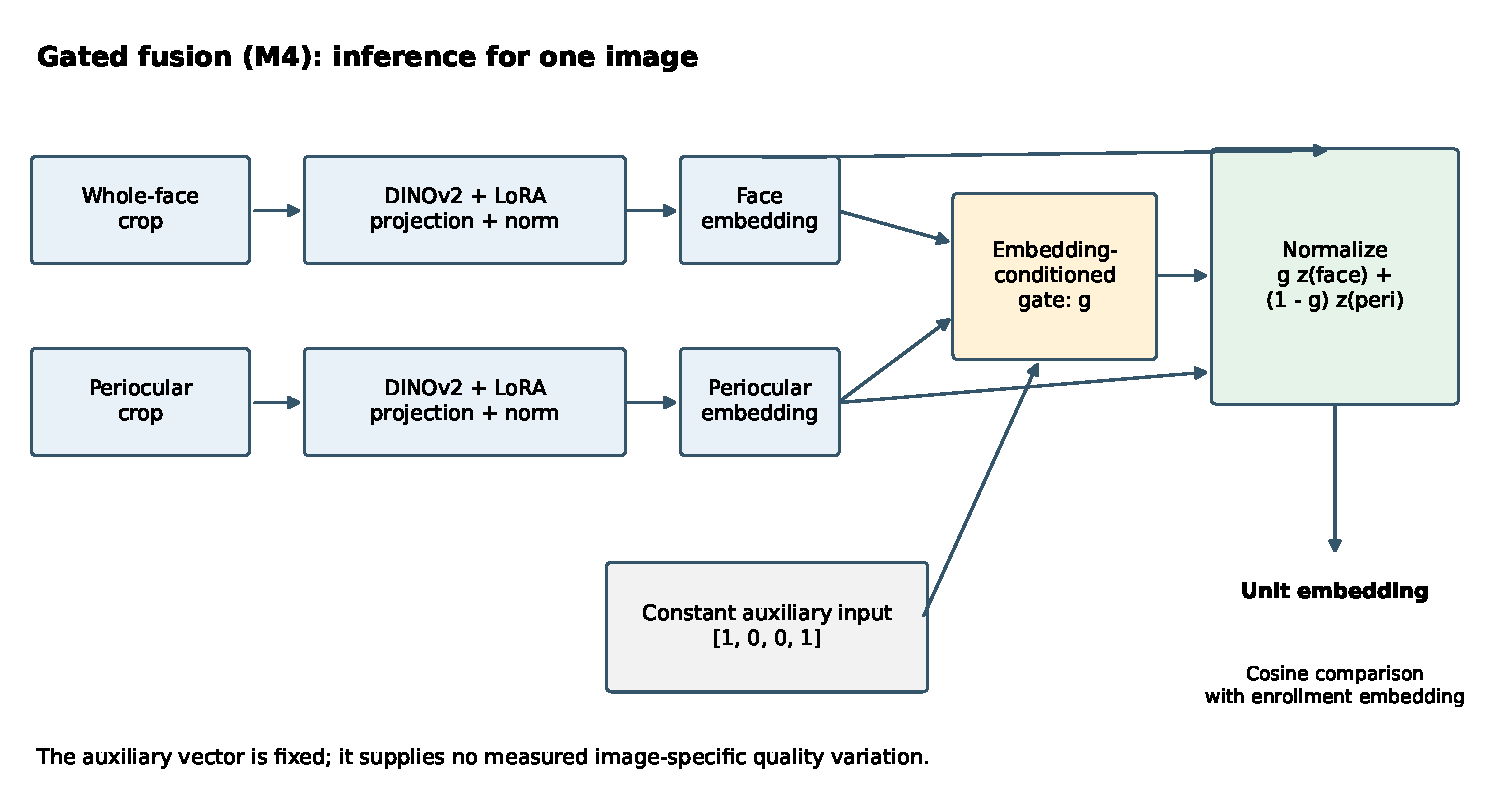
\includegraphics[width=0.98\textwidth]{fig_gated_architecture.pdf}
\caption{The auxiliary vector contains no image-specific quality variation. The embeddings from both branches, along with the constant auxiliary vector, are passed into the gated sum. The weighted sum is normalised. The same model processes the enrolment image. During inference, the training-only identity classifier has been removed.}\label{fig:supparchitecture}\end{figure*}

\section{Shared-crop preprocessing for SFace}

The exact DINOv2 full face files were scaled to 112x112 to create SFace images, with no YuNet detection or landmark alignment. AUC values of 0.8408, 0.7775, 0.8689, 0.9513 and 0.6532 were found for masked ROF, sunglasses ROF, neutral ROF, MFR2 and RMFRD, respectively (Supplemental Table S3). Features were extracted successfully from all 3402 unique images. Due to differing preprocessing between protocols, the AUC values cannot be considered directly comparable baseline values. Neither protocol is a matched-training comparison with DINOv2 due to differences in architecture, pre-training, resolution and supervision.\par

\begin{table}[!ht]\centering\footnotesize\setlength{\tabcolsep}{2pt}
\caption{AUCs from different preprocessing protocols applied to SFace. All pairs affected by detection or embedding failure are included in AUC with score -1. The number of failed pairs per protocol is shown. Only the aligned diagnostic results are shown in Table IX in the main text.}
\label{tab:sfaceshared}\begin{tabular}{lrrrr}\toprule
Protocol & Aligned AUC & Failed & Shared AUC & Failed\\\midrule
Masked ROF & 0.9399 & 9 & 0.8408 & 0\\
Sunglasses ROF & 0.9440 & 48 & 0.7775 & 0\\
Neutral ROF & 0.9991 & 0 & 0.8689 & 0\\
MFR2 & 0.9968 & 0 & 0.9513 & 0\\
RMFRD & 0.8187 & 1155 & 0.6532 & 0\\
\bottomrule\end{tabular}\end{table}

\section{Provenance}

Data from existing sources have been used within this project (ROF, MFR2, RMFRD). The Kaggle execution copies can be identified from the project records. The source data can be found in the ROF and RMFRD repositories and the MFR2 maintainer page. The local ROF annotation files match the audited source files. A complete trace as to how the images were obtained was not able to be found. Identifiers relating to source data and exclusion ledgers remain.\par

Within the ROF repository, software and documents are licensed under MIT. In the MFR2 maintainer page, Creative Commons licensing is mentioned but no further details on the type or terms of the licence are given. In the RMFRD README, it is stated that the data was obtained from online sources. No clear licence information was found, however, regarding using the images. As such, it cannot be confirmed with certainty that all images used within this project have the correct licensing to be used, nor that the redistribution rules are definitively applicable to all images. Source faces and trained model checkpoints are not included in this release. Source code, manifests, hashes, derived scores and figures from the manuscript are included.\par

The author confirms that no ethics committee reviewed this project. No formal approval or exemption is claimed. The public records reviewed do not establish individual participant consent or complete image-use permissions. From publicly available data, no approval numbers, waivers, consents or general permission to use images within the data can be inferred. The applicable ethics-review requirement and image-use permissions remain unverified.\par

Source records checked on 22 November 2026: \href{https://github.com/ekremerakin/RealWorldOccludedFaces}{ROF repository}, \href{https://github.com/ekremerakin/RealWorldOccludedFaces/blob/main/LICENSE}{ROF licence}, \href{https://sites.google.com/view/masktheface/mfr2-dataset}{MFR2 maintainer page}, \href{https://github.com/X-zhangyang/Real-World-Masked-Face-Dataset}{RMFRD repository}.\par
\end{document}
